\chapter{Methodology for Conducting Nonlinear Time Reversal}
\label{ch:nonlinear-meth}

To reference this figure type ...in Figure~\ref{fig:nonlinear-diagram}. Note that the tilde is attached to the word figure, no space.

\begin{figure}[h!]
\centering
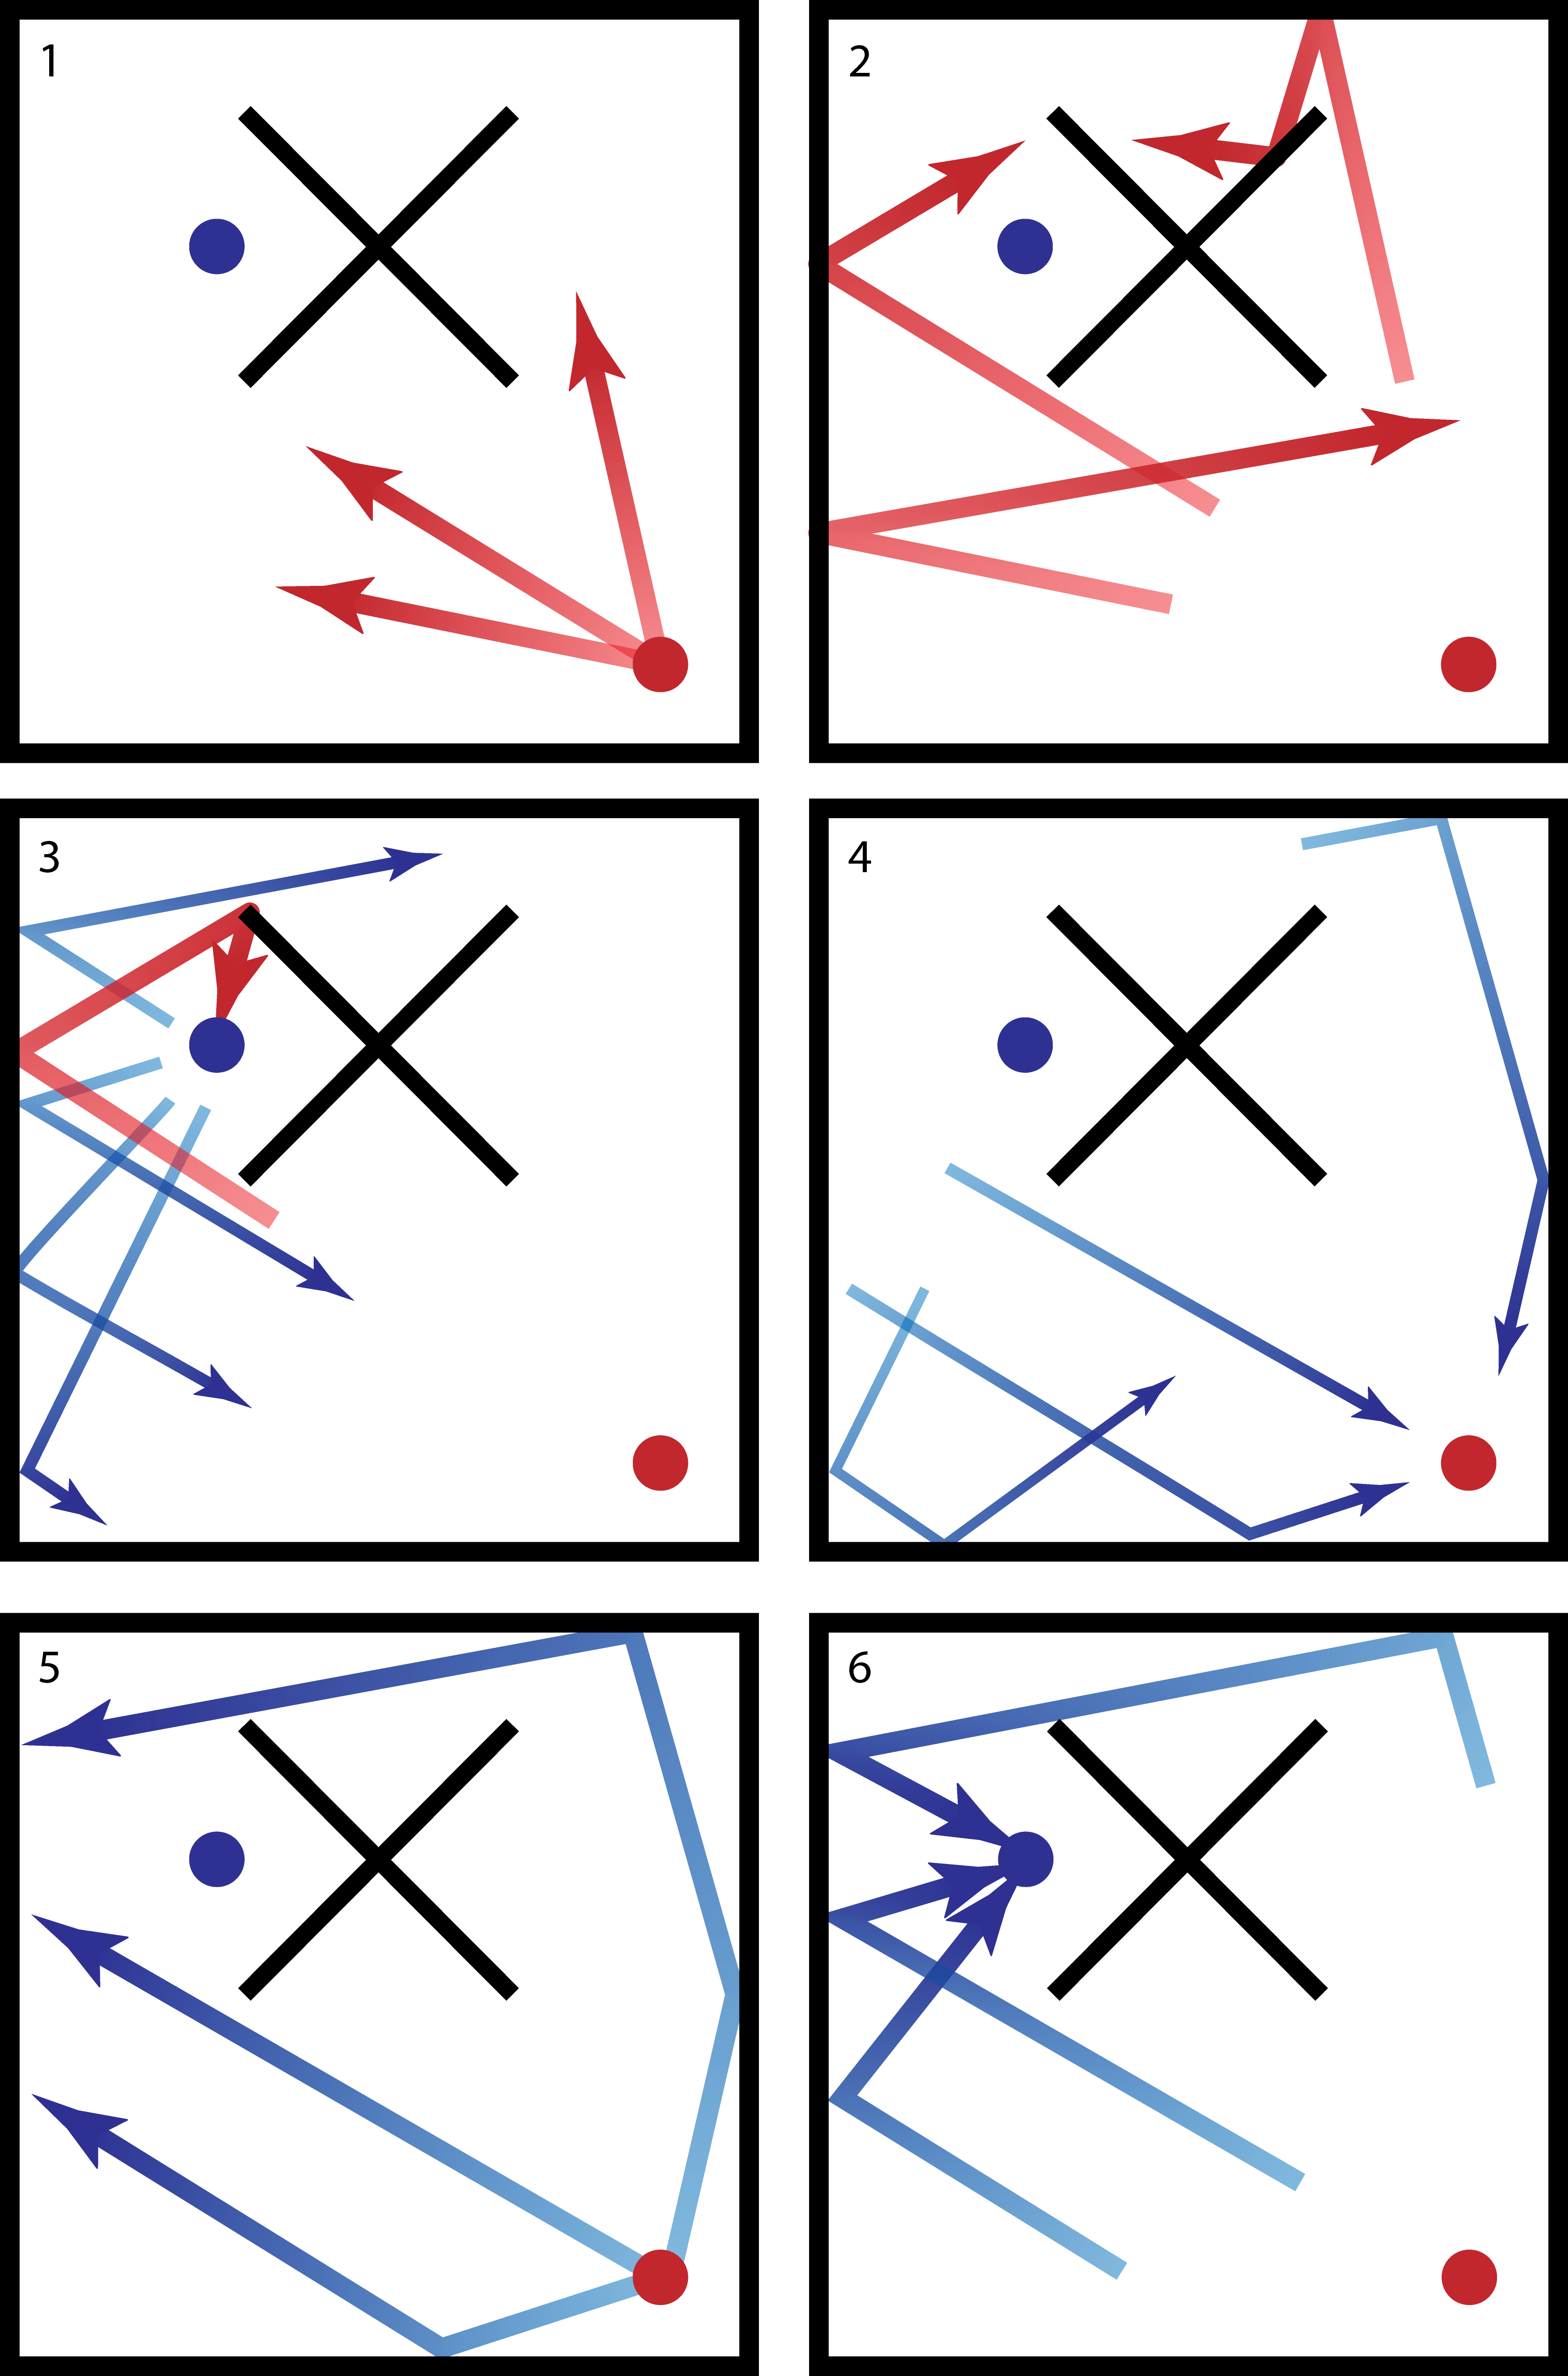
\includegraphics[width=0.85\textwidth]{nonlinear/diagram}
    \caption[Demonstration of nonlinear time reversal]{Reading order from top left: 1) The TRM broadcasts a signal into the cavity at one frequency, which 2) reverberates within the cavity. Eventually, 3) the signal reaches the nonlinear element somewhere within the chamber. Reflected waves that encounter this element will have a characteristic frequency signature containing harmonics of the original signal. 4) Some of these harmonic reflections will find their way back to the TRM. The TRM filters the sona to extract only those reflections, then time reverses and 5) re-emits them. 6) The time reversed waves collapse back on the nonlinear target.}
    \label{fig:nonlinear-diagram}
\end{figure}